\chapter{Off-Chain Design}
\label{chap:offchainDesign}
In this chapter, we present the design of the of-chain components of the \acrlong{ew} environment, which have been developed to offer a user-friendly interface for stakeholders and support the integration of system functionalities. Together with the smart contracts described in \cref{chap:onchainDesign}, these components form the complete system architecture, as illustrated in \cref{fig:fullArchDiag}. 

\begin{figure}[htpb]
  \centering
  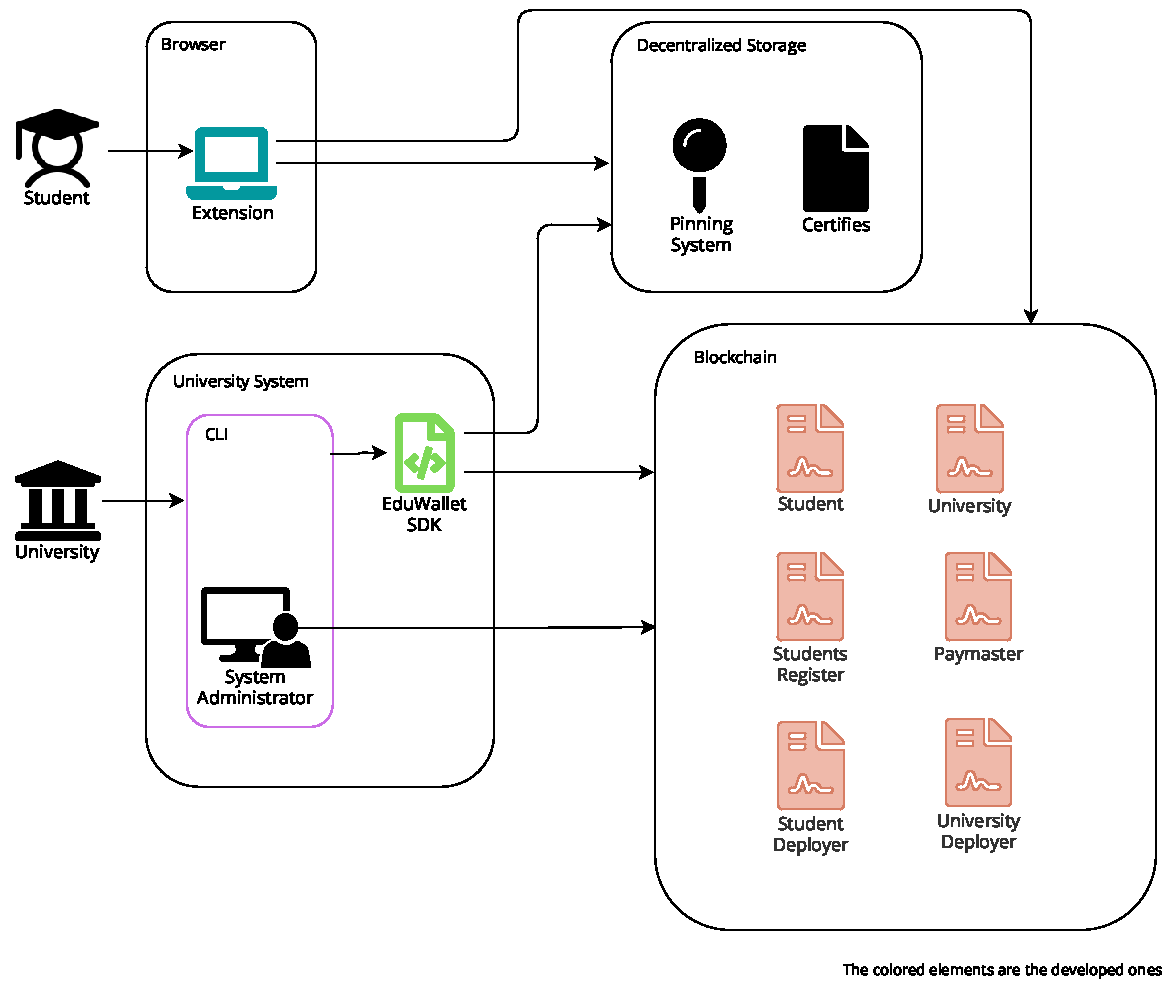
\includegraphics[width=0.8\textwidth]{figures/Architecture diagram complete.pdf}
  \caption[System architecture diagram]{Complete architecture of the \acrlong{ew} system}
  \label{fig:fullArchDiag}
\end{figure}

Given that students using \acrshort{ew} are not expected to have expertise in blockchain technologies, the platform must provide a simple yet effective interface. This interface should enable them to interact with their academic wallets, retrieve academic results, and manage access permissions. These requirements are address \textit{FR 11} in \cref{tab:funcReq}. Similarly, smart contracts interactions may pose challenges even for universities and their \acrfull{it} departments. Therefore, the system must also offer a simplified and accessible interface for institutional use, as specified in \textit{FR 8} in \cref{tab:funcReq}. 
To satisfy these usability needs, two primary components were developed: a \textbf{browser extension} for student interactions with their academic wallets, and a \textbf{\acrlong{sdk}} designed to facilitate the integration of \acrshort{ew} within university systems.

Moreover, \textit{NFR 3} in \cref{tab:nonFuncReq} emphasizes the need to minimize on-chain storage consumption and associated costs by limiting blockchain use to essential data only. To support this goal, the system incorporates a \textbf{decentralized storage} solution, which is responsible for storing and providing access to large data files, such as academic certificates and other supporting documentation.

Finally, to enable comprehensive testing of the environment, a \textbf{\acrlong{cli}} was developed. This tool simulates a real university \acrshort{lms} and allows for testing the \acrshort{sdk} functionalities, as well as its interaction with smart contracts and the decentralized storage layer.

%%%%%%%%%%%%%%%%%%%%%%%%%%%%%%%%%%%%%%%%%%%%%%%%%%%%%%%%%%%%%%%%%%
% BROWSER EXTENSION
%%%%%%%%%%%%%%%%%%%%%%%%%%%%%%%%%%%%%%%%%%%%%%%%%%%%%%%%%%%%%%%%%%
 \section{Browser Extension}
\label{sec:browserExtensionDesign}
This section presents the browser extension, which serves as the primary interface for students to interact with their academic wallets. Its main objective is to abstract the complexity of on-chain operations by offering a user-friendly interface that aligns with the design and usability standards of traditional web applications, addressing \textit{FR 11} in \cref{tab:funcReq}.

\subsection{Technological Choices}
To achieve the highest level of decentralization and autonomy for users, we chose to implement a browser extension rather than a traditional web application. Conventional web applications, typically accessed via a \acrshort{url}, rely on a server to host both the user interface (front-end) and the business logic (back-end), but this architecture introduces central points of control and potential failure. Such reliance would conflict with \textit{NFR 6} in \cref{tab:nonFuncReq}, which emphasizes the importance of minimizing centralization within the system's design.
In contrast, a browser extension operates more like a lightweight desktop application, but within the browser environment. This eliminates the need for an external server to host the interface and, since the core logic of the \acrlong{ew} system resides in smart contracts deployed on the blockchain, no additional server-side back-end is required. This architecture ensures that both the user interface and the underlying logic remain fully decentralized, depending only on the local extension and on-chain infrastructure.
Beyond decentralization, browser extensions offer a compact, wallet-like user experience. Rather than a full screen web page, they present a small, easily accessible window via an icon in the browser toolbar. This interaction model is common among cryptocurrency wallets, such as MetaMask, offering users an intuitive means of managing on-chain assets. Adopting the same paradigm for academic records helps students access and control their data seamlessly, reinforcing the concept on an academic wallet.

Browser extensions are supported across several major browsers, including Microsoft Edge, Google Chrome and Firefox. While each browser introduces minor platform-specific differences, we opted to develop the extension primarily for Google Chrome. Chrome currently holds the largest global browser market share\footnote{\url{https://en.wikipedia.org/wiki/Usage_share_of_web_browsers}}, offering a broad potential user base. Additionally, since Google Chrome and Microsoft Edge are both based on the Chromium open-source project, extensions developed for Chrome are also compatible with Microsoft Edge, further extending platform reach without additional development overhead.

Among the various technologies available for browser extensions development, we selected TypeScript as the core programming language and React as the framework for building the user interface. TypeScript offers the flexibility and web-centric capabilities of JavaScript while introducing static typing, which improves code safety, clarity, and maintainability. It also integrates seamlessly with smart contract development, as libraries exist to generate TypeScript types directly from contract definitions.
React, originally developed by Facebook as an open-source JavaScript library, is widely used for building modern web interfaces. It enables efficient \acrshort{ui} development and facilitates seamless interaction with application logic.
Our familiarity and prior experience with both React and JavaScript also influenced our choice, enabling a faster and more reliable development process. Additionally, we employed \textit{Vite} as the building tool for our environment, making it easier to manage and bundle the various modules of our browser extension efficiently.

\subsection{Functionalities}
\label{ssec:extFunctionalities}
The browser extensions provides students with all necessary tools to access and manage their academic wallets. The primary entry point is the login functionality. To authenticate, students enter the credentials (see \cref{fig:loginExtDesign}) supplied by the university at wallet creation. During login, the extension derives the private key of an \acrshort{eoa} from the student's ID and password using the PBKDF2 algorithm. PBKDF2 is a key-derivation function that, given a \gls{salt} and a password, produces the private key of an \acrlong{eth} \acrlong{eoa}. In our implementation, the student's ID serves as the \gls{salt}, eliminating the need for a centralized \gls{salt} repository and ensuring uniqueness per users. Upon deriving the private key and instantiating the \acrlong{eoa}, the extension queries the StudentsRegister contract to retrieve the associated \acrlong{sca} address. If a valid address is returned, authentication succeeds and the extension proceeds to fetch the student's personal details and academic records from their smart account.

\begin{figure}
  \centering
  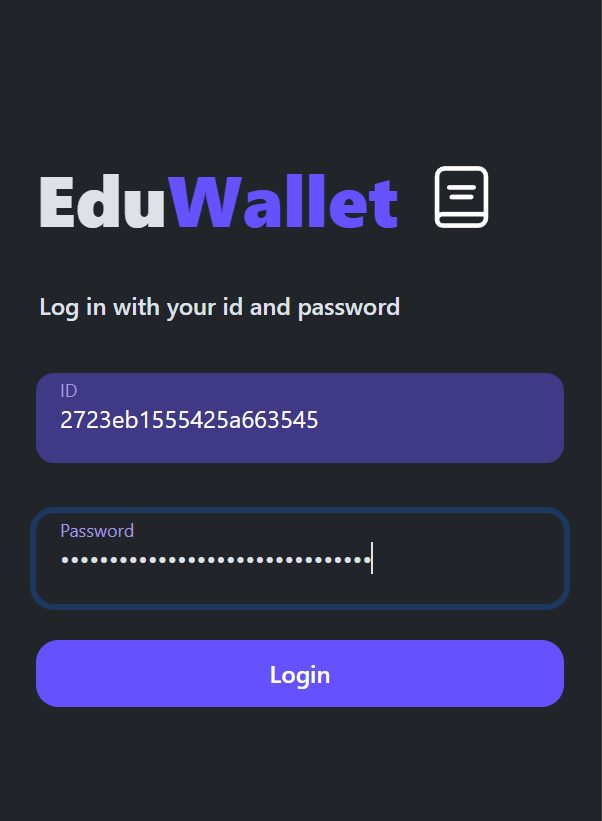
\includegraphics[width=0.45\textwidth]{figures/Login.png}
  \caption[Browser extension login page]{Screenshot of the browser extension login window.}
  \label{fig:loginExtDesign}
\end{figure}

Once logged in, students can view a consolidated list of their academic records (\cref{sfig:homepageExt}) and inspect individual entries (\cref{sfig:singleRecordExt}). Records are grouped first by university, using each institution's short identifier, and then by degree program. Each entry displays the course name, course code, \acrshort{ects} credits, and grade, if available. The homepage also shows the student's total accumulated \acrshort{ects}. Selecting a record opens its detailed view, which adds the date of evaluation and hyperlink to the certificate stored on the decentralized storage system. 

\begin{figure}
    \centering
    \begin{subfigure}{.45\textwidth}
        \centering
        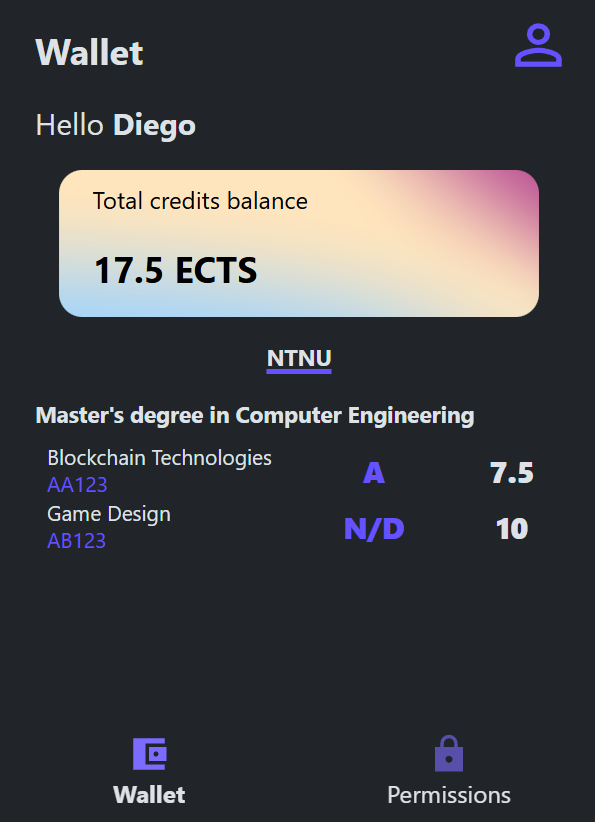
\includegraphics[width=\textwidth]{figures/Homepage.png}
        \caption{Homepage}
        \label{sfig:homepageExt}
    \end{subfigure}
    \hfill
    \begin{subfigure}{.45\textwidth}
        \centering
        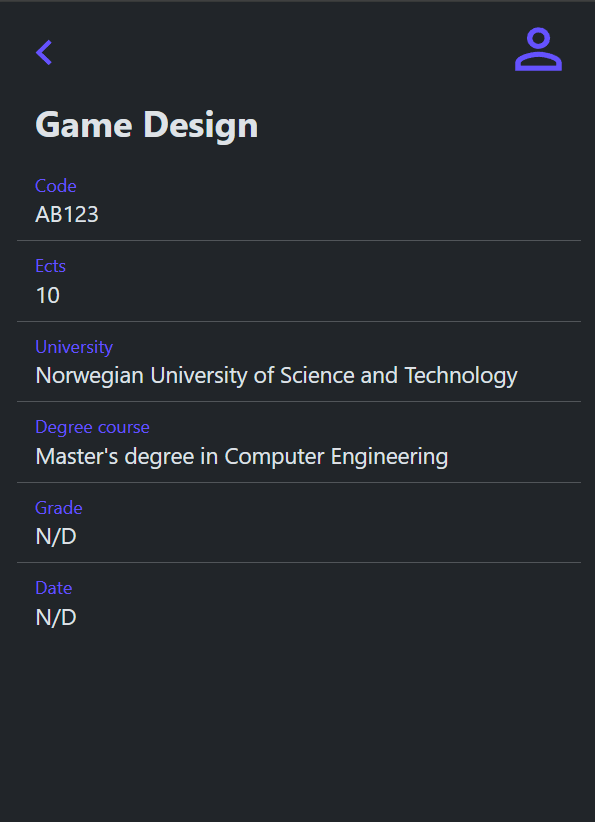
\includegraphics[width=\textwidth]{figures/SingleCourse.png}
        \caption{Single record page}
        \label{sfig:singleRecordExt}
    \end{subfigure}
    \caption[Browser extension windows for academical records]{Screenshots of the browser extension showing the academic records homepage and detailed record view.}
    \label{fig:recordsExt}
\end{figure}

The extension also supports permission management via the lock icon. In this interface (\cref{fig:permissionsExt}), students can review granted permission and pending access requests from universities. The permissions are categorized into three groups: requests, read permissions and the write permissions. Buttons adjacent to each entry enable students to easily grant new permissions or revoke existing ones, ensuring full control over their academic wallet.

\begin{figure}
  \centering
  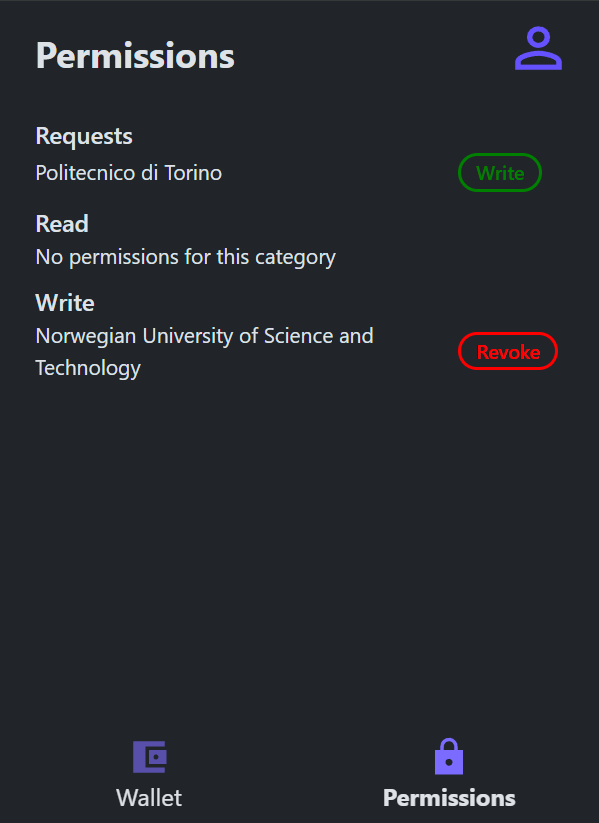
\includegraphics[width=0.45\textwidth]{figures/Permissions.png}
  \caption[Browser extension permissions page]{Screenshot of the extension permissions window.}
  \label{fig:permissionsExt}
\end{figure}

Finally, clicking the user icon in the top‐right corner opens the personal information page, where students can view their profile details (\cref{fig:userInfoExt}).

\begin{figure}
  \centering
  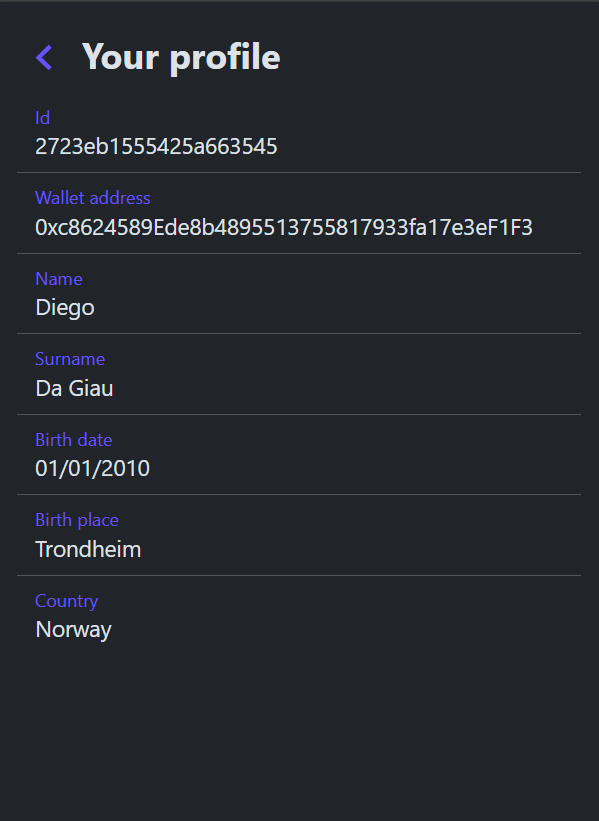
\includegraphics[width=0.45\textwidth]{figures/PersonalInfo.png}
  \caption[Browser extension user information page]{Screenshot of the browser extension user information window.}
  \label{fig:userInfoExt}
\end{figure}

\subsection{Blockchain Interactions}
\label{ssec:extBlockchainInteraction}
The most straightforward way to perform on-chain operations from off-chain components is by using external libraries specifically designed to streamline these interactions. The two primary options are \textit{web3}\footnote{\url{https://web3js.readthedocs.io/en/v1.10.0/index.html}} and \textit{ethers}\footnote{\url{https://docs.ethers.org/v6/}}. We opted for \textit{ethers} over \textit{web3} because it is more lightweight, an essential feature for web applications that must minimize browser resource usage, and because it is more modern and offers better TypeScript support. 
Another crucial library used in the development of the extension is \textit{TypeChain}, a TypeScript-oriented tool that, given the Solidity code of smart contracts, extracts type definitions that can be imported directly into the application. This ensures our application remains type-safe and consistent with the structures and requirements defined in the smart contracts that comprise \acrlong{ew}. 

With these libraries in place, the browser extension needs to establish a connection to the blockchain to execute operations. Our system leverages the \textit{ethers} JSON-RPC provider, which connects to a chain via its \acrshort{url}. The \acrshort{url} of the used chain is hardcoded in the extension, along with the addresses of the core contracts, namely, the StudentsRegister, EntryPoint and Paymaster (see \cref{lst:confExt}). To deploy the extension on a different configuration, such as a layer 2 network with a new \acrshort{url} and different core contract addresses, these values must be manually updated in the extension's source code.

\lstinputlisting[
    caption={Blockchain configuration info data variable and its type definition},
    label=lst:confExt,
    language=TypeScript
]{listings/conf.ts}

To support the required on-chain functionalities, the browser extension performs three types of interactions:
\begin{enumerate}
    \item Direct read-only operations
    \item Read-only operations via the \acrlong{sca}
    \item Transactions via the smart account
\end{enumerate}

\subsubsection{Direct Read-Only Operation}
This is the simplest interaction and is executed, for example, during login phase, where the extension retrieves the address of the student's smart account. In this case, the extension directly invokes the corresponding function of the StudentsRegister contract, using the student's \acrshort{eoa} as the sender. 

\subsubsection{Read-Only Operation via Smart Account}
These interactions occur when retrieving permissioned data, such as academic records, accessible only to authorized universities or the student. For this, the extension invokes the dedicated function to execute read-only operations, provided by the SmartAccount contract. As described in \cref{sec:smartAccountDesign}, the call requires specifying:

\begin{itemize}
    \item the address of the target contract
    \item the encoded function signature and parameters (call data)
\end{itemize}
Encoding is handled using functions from the \textit{ethers} library. The operation is executed using the student's \acrshort{eoa}.

\subsubsection{Transaction via Smart Account}
This type of interaction is required for operations that alter blockchain state, such as granting or revoking permissions to universities, by accessing restricted functions. These actions require gas consuming transaction executed via the student's \acrlong{sca}, using UserOperations.
The browser extension constructs a UserOperation by assembling the following fields:
\begin{itemize}
    \item Sender address (the student's \acrshort{eoa} address)
    \item Target contract address
    \item Encoded function name and parameters
    \item Gas and fee-related parameters
    \item Transferred value (always set to 0 in our case)
    \item Paymaster address and associated parameters
    \item Student's \acrshort{eoa} signature, generated using \textit{ethers} utilities
\end{itemize}
After constructing the UserOperation, the extension sends it directly to the EntryPoint contract using its hardcoded address. As discussed in \cref{ssec:accountAbstraction}, in a public network deployment, this operation would be relayed via a bundler instead.

\subsection{UI Prototyping}
The \acrlong{ui} was initially designed using \textit{Figma}, a powerful prototyping tool that enables detailed visualization and planning \acrlong{ui} across various types of applications. The \acrshort{ui} prototype, accessible via the link provided in \cref{chap:figma}, played a crucial role not only in shaping the visual layout of the extension, but also in refining its functional requirements. 
By sketching out all application windows and placing ourselves in the shoes of end users, we were able to identify the key pieces of information the interface needed to convey and determine the most effective ways to present them. 

%%%%%%%%%%%%%%%%%%%%%%%%%%%%%%%%%%%%%%%%%%%%%%%%%%%%%%%%%%%%%%%%%%
% SDK
%%%%%%%%%%%%%%%%%%%%%%%%%%%%%%%%%%%%%%%%%%%%%%%%%%%%%%%%%%%%%%%%%%
\section{Software Development Kit}
\label{sec:sdkDesign}
This section describes the \acrlong{sdk}, a TypeScript package designed to simplify integration of the \acrlong{ew} system within university infrastructure. By abstracting low-level blockchain concerns, such as \acrshort{eoa} key management, contract deployment and referencing, read-only queries and gas consuming transactions, the \acrshort{sdk} lowers the barrier to entry for institutions wishing to adopt on-chain academic records.

When evaluating integration strategies, we considered two alternatives: web \acrshort{api}s and a stand-alone \acrshort{sdk}. Web \acrshort{api}s require a centralized server to receive client requests, execute business logic, and relay blockchain interactions. In contrast, an \acrshort{sdk} is distributed as a client-side library that runs directly within the user's environment, requiring no dedicated server infrastructure beyond standard package hosting. This approach aligns with \textit{NFR 6} in \cref{tab:nonFuncReq}, which prioritizes decentralization.
Moreover, an \acrshort{sdk} offers superior scalability compared to \acrshort{api}s. Since \acrshort{api} calls traverse the public internet and share server resources, they can be affected by network latency or server overload when serving thousands of institutions worldwide. The \acrshort{sdk}, by running locally on each institution's system, minimizes network dependencies and leverages the user's own compute resources.
However, \acrshort{sdk}s entail two main trade-offs. First, updates depend on consumer upgrading to newer package versions, whereas a centralized \acrshort{api} can be improved transparently. Second, \acrshort{sdk}s are inherently platform-specific: a TypeScript \acrshort{sdk} supports only JavaScript/TypeScript environments. To address this, one must develop and maintain multiple \acrshort{sdk} variants for different languages or platform.

Given that our off-chain components are implemented in TypeScript, and that Node.js\footnote{An open-source server environment used to run JavaScript and TypeScript code outside the browser (\url{https://nodejs.org})} is widely adopted in modern back-end systems, we selected TypeScript for the \acrshort{sdk}. The choice maximizes compatibility with university \acrshort{it} stacks and leverages existing expertise in the JavaScript ecosystem.

\subsection{Working with the SDK}
Once imported in the university's system, the \acrshort{sdk} exposes a suite of functions and types that encapsulate all interaction with the on-chain academic record platform. An example of its usage is shown in \cref{lst:sdkCall}, where the \acrshort{sdk} is imported and used to register a student in the system. The registration function accepts two parameters: the university \acrshort{eoa} wallet, instantiated from the private key provided at university enrolment using the \textit{ethers} \texttt{Wallet} type; and a \texttt{StudentData} object, a type defined by the SDK that includes the student’s name, surname, date of birth (YYYY-MM-DD), place of birth, and country of birth. The function returns the student's credentials (ID and password) and the \acrshort{sca} address. Because all \acrshort{sdk} calls involve blockchain queries or transactions, each function is declared asynchronous and must be awaited by the caller.

\lstinputlisting[
    caption={Import of the \acrshort{sdk} and exemplar invoke},
    label=lst:sdkCall,
    language=TypeScript
]{listings/sdkCall.ts}

In addition to students registration, the \acrshort{sdk} provides the following core functionalities for university integrators:
\begin{itemize}
    \item Enrol a student in one or more courses.
    \item Record a new evaluation for a student.
    \item Retrieve a student’s personal details.
    \item Retrieve a student’s personal details and complete academic records.
    \item Request permission to read from or write to a student’s academic wallet.
    \item Verify an existing permission in a student’s academic wallet.
\end{itemize}

\subsubsection{Register a student}
Universities register students by providing their own \acrshort{eoa} and a \texttt{StudentData} object. The \acrshort{sdk} generates a new \acrshort{eoa} for the student using PBKDF2 algorithm, already presented in \cref{ssec:extFunctionalities}. Specifically, the \acrshort{sdk} randomly generates a student's ID and password, which are used as inputs to derive the private key. This approach satisfies \textit{NFR 1} in \cref{tab:nonFuncReq} by avoiding reliance on third-party wallets (e.g., MetaMask). The \acrshort{sdk} then constructs a UserOperation to invoke the registration function on the StudentsRegister contract via the university's smart account. Finally, it queries the StudentsRegister to retrieve the student's \acrshort{sca} address and returns it, along with the student's credentials, to the caller.

\subsubsection{Enrol a student}
To enrol students in courses, the \acrshort{sdk} requires the university's \acrshort{eoa} wallet, the student's \acrshort{sca} address, and an array of \texttt{CourseInfo} objects, each containing course code, name, degree program, and \acrshort{ects} credits. The \acrshort{sdk} converts these into the format expected by the Student contract's \texttt{Result} structure (\cref{sec:studentContract}) and submits a UserOperation to perform the enrolment.

\subsubsection{Record a new evaluation}
Recording an evaluation requires the university’s \acrshort{eoa} wallet, the student’s \acrshort{sca} address, and an array of \texttt{Evaluation} objects. Each object includes the course ID, grade, evaluation date, and an optional path to a certificate file. For entries that include certificates, the \acrshort{sdk} first uploads the file to the decentralized storage system (see \cref{sec:decStorageDesgn}) and retrieves a reference to it. It then assembles a UserOperation containing all relevant data, including the storage reference. This UserOperation is executed via the university's smart account to invoke the evaluation function in the student's \acrshort{sca}.

\subsubsection{Retrieve Student Details and Records}
To fetch personal details, with or without academic records, the \acrshort{sdk} takes the university's \acrshort{eoa} wallet and the student's \acrshort{sca} address. It executes a read-only operation via the university's \acrshort{sca}, to invoke the appropriate view function on the student's smart account. Upon success, the \acrshort{sdk} maps the returned data into a \texttt{Student} object, containing \texttt{StudentData} and an array of academic records.

\subsubsection{Request a permission}
When a university needs permission to read or write a student’s academic wallet, the SDK requires the university’s \acrshort{eoa} wallet, the student’s \acrshort{sca} address, and the desired permission type (\texttt{Read} or \texttt{Write}). It then constructs and submits a UserOperation to call the corresponding function on the student’s \acrshort{sca}.

\subsubsection{Verify permissions}
To verify existing permissions, the \acrshort{sdk} takes the university's \acrshort{eoa} wallet and the student's \acrshort{sca} address. It then executes a read-only operation via the university's smart account, targeting the student smart account. The student's \acrshort{sca} returns the granted permission type, or null if none is held. The \acrshort{sdk} forwards this result to the caller, using the appropriate TypeScript type.

\subsection{Access On-Chain Functionalities}
Since the \acrshort{sdk} adopts the same model as the browser extension to access on-chain functionalities, the \cref{ssec:extBlockchainInteraction} provides a thorough explanation of the different types of interactions, as well as the tools and libraries used to execute them.

\subsection{Input Management}
All the \acrshort{sdk} functions perform input validation and presence check to ensure data integrity. For instance, the function responsible fro registering a new evaluation in a student's academic wallet first verifies that all requires parameters are provided. It then checks whether the student's smart account address is valid by confirming it begins with '0x'. This function also ensures that the array of evaluations contains at least one entry and, for each evaluation, verifies the presence of all mandatory fields.

%%%%%%%%%%%%%%%%%%%%%%%%%%%%%%%%%%%%%%%%%%%%%%%%%%%%%%%%%%%%%%%%%%
% DECENTRALIZED STORAGE SYSTEM
%%%%%%%%%%%%%%%%%%%%%%%%%%%%%%%%%%%%%%%%%%%%%%%%%%%%%%%%%%%%%%%%%%
\section{Decentralized Storage System}
\label{sec:decStorageDesgn}
This section presents our solution to one of the most significant challenges in blockchain-based systems: the high cost of on-chain storage. To address this issue, presented also through the \textit{NFR 3} in \cref{tab:nonFuncReq}, we introduce an off-chain decentralized storage solution in our project. This system is used to store and retrieve certification files, such as language certificates or graduation diplomas, which require significantly more space than plain text\footnote{PDF files typically range from a few kilobytes to several megabytes, whereas plain text data usually occupies only a few bytes.}. Storing such documents directly on-chain would result in substantial gas costs, making the approach impractical. 

We chose a decentralized storage system over traditional local or cloud-based solutions to maintain the decentralized nature of our environment and to meet \textit{NFR 6} outlined in \cref{tab:nonFuncReq}. Among the various decentralized options available, we selected \acrfull{ipfs} for its ability to provide verifiable and distributed file storage. This choice is motivated by several factors: \acrshort{ipfs} is an open source protocol with a large and active community, strong support, and widespread adoption. It also serves as the foundational layer for many other decentralized platforms, such as Filecoin\footnote{\url{https://filecoin.io}} and Web3.Storage\footnote{\url{https://web3.storage}}, allowing future extensions or upgrades to be implemented with minimal effort \cite{erikflorian2022ipfsandfrineds}. Furthermore, \acrshort{ipfs} ensures immutability of stored files, a critical feature for academic certificates, which must remain unchanged over time.

\subsection{Pinning files}
To fully leverage \acrshort{ipfs}, we integrated Filebase\footnote{\url{https://filebase.com}}, a third-party pinning service. Pinning refers to the act of instructing a node to keep a copy of a file permanently, preventing it from being removed during garbage collection. Without Filebase, we would have needed to run our own local \acrshort{ipfs} node and manage file pinning manually, an approach that introduces instead complexity, higher maintenance costs, and reduced data availability in a testing system like ours. In contrast, Filebase handles node operation and file pinning, offering an accessible solution thorough its AWS S3-compatible \acrshort{api}, which simplifies file uploads to the peer-to-peer network. Notably, Filebase also provides a free tier allowing up to 5 GB of storage, which is sufficient for our needs. This is an advantage over other pinning solutions such as Web3.Storage, which lacks a fully free plan, or Pinata\footnote{\url{https://pinata.cloud}}, which offers more limited options.

\subsection{Integration in the system}
As illustated in \cref{fig:fullArchDiag}, both the browser extension and the \acrshort{sdk} interact with the storage system. The browser extension enables students to retrieve certificates associated with their academic records through the official \acrshort{ipfs} public gateway. As shown in \cref{fig:courseWithCertificate}, each certificate is presented as clickable, composed by the gateway's base \acrshort{url} followed by the file's \acrfull{cid} on the \acrshort{ipfs} network. The \acrshort{cid} of each document is stored on-chain within the student's academic wallet, alongside other record information such as the course name (see \cref{sec:studentContract}). This enables students to view and download their certificates from a standard web interface.

\begin{figure}
  \centering
  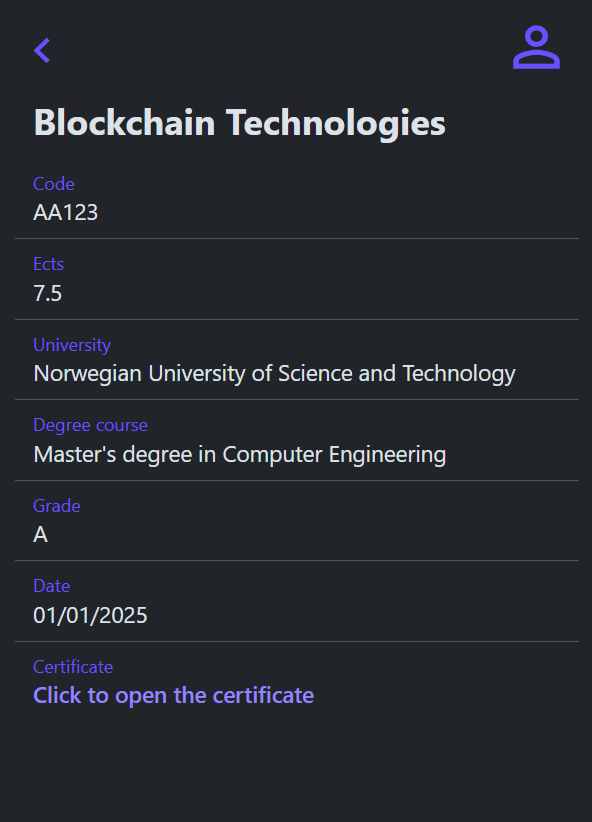
\includegraphics[width=0.45\textwidth]{figures/SingleCourseWithCertificate.png}
  \caption[Browser extension screenshot with certificate link]{Screenshot of the browser extension presenting the page of a course. The image shows the link to the certificate saved in the decentralized storage.}
  \label{fig:courseWithCertificate}
\end{figure}

Similarly, the \acrshort{sdk} uses the same mechanism to retrieve certificates on behalf of universities. When uploading a file, however, the \acrshort{sdk} interacts directly with Filebase to ensure the file is pinned and hosted by an active node. The \acrshort{sdk} receives the document from the university, then uses the AWS S3-compatible \acrshort{api} to upload it. The \acrshort{api} requires the key associated with the pinning account (managed by the \acrshort{ew} system administrator) and the file itself. In return, it provides the \acrshort{cid}, which is then stored in the academic record.
% TODO: Reference implementation section

\subsection{Security and Limitations}
Academic certifies, and official documents more broadly, are legal artifacts that must always be secure and verifiable. \acrshort{ipfs} inherently supports these properties through its use of content-based addressing. In this model, each file is identified by a \acrshort{cid}, which is derived from the cryptographic hash of the file's content. Any alteration to the file results in a completely different \acrshort{cid}, ensuring that tampering is immediately detectable \cite{benet2014ipfscontentaddressed}. Since the \acrshort{cid} is stored on the blockchain at the time the certificate is issued by the university, the document's authenticity and integrity are guaranteed.

While \acrshort{ipfs} offers strong immutability and verifiability, it lacks built-in access control. In the context of our system, we assume that certificates are publicly accessible documents. Consequently, any part in possession of a file's \acrshort{cid} can retrieve it via the public gateway. However, if access control becomes a requirement, there are several strategies to address this limitation \cite{barbaraanrealaura2021datapersistence}. One option is to encrypt files before uploading them to \acrshort{ipfs}, such that only authorized components within our system can decrypt them. Another approach is to use a private \acrshort{ipfs} network, where access can be restricted to approved entities. The trade-offs and potential implications of such private deployment will be discussed in the FUTURE\_WORK\_REFERENCE.

%%%%%%%%%%%%%%%%%%%%%%%%%%%%%%%%%%%%%%%%%%%%%%%%%%%%%%%%%%%%%%%%%%
% CLI
%%%%%%%%%%%%%%%%%%%%%%%%%%%%%%%%%%%%%%%%%%%%%%%%%%%%%%%%%%%%%%%%%%
\section{CLI}
\label{sec:cliDesign}
This section describes the testing tool developed to evaluate the use of the \acrshort{sdk}. In a real-world deployment, universities are expected to integrate the \acrshort{sdk} into their existing \acrshort{lms} to interact with \acrlong{ew}. However, given that this is a testing environment, smaller and simpler than a real-world deployment, we developed a minimal \acrlong{cli} to simulate the interaction between a university's system and our academic register. We opted to implement a CLI rather than a web application or desktop GUI and this decision allowed for faster development, enabling us to focus on the core functionalities of the \acrshort{sdk}, the blockchain logic, and the browser extension, without introducing additional complexity related to graphical or \acrfull{ux} design.

\cref{fig:clifigs} illustrates the visual aspects of the \acrshort{cli}. In \cref{sfig:cliDesign1}, users can navigate through a sliding menu offering various options. When input is required, the interface prompts the user for the necessary information and provides visual feedback upon completion of the operation (\cref{sfig:cliDesign2}).The \acrshort{cli} leverages the \textit{inquirer}\footnote{\url{https://www.npmjs.com/package/inquirer}} TypeScript library to manage user interactions and uses \textit{ora}\footnote{\url{https://www.npmjs.com/package/ora}} to display feedback. Specifically, \textit{ora} is responsible for showing success and error messages, as well as animated text with spinners to indicate ongoing operations.

\begin{figure}
    \centering
    \begin{subfigure}{.5\textwidth}
        \centering
        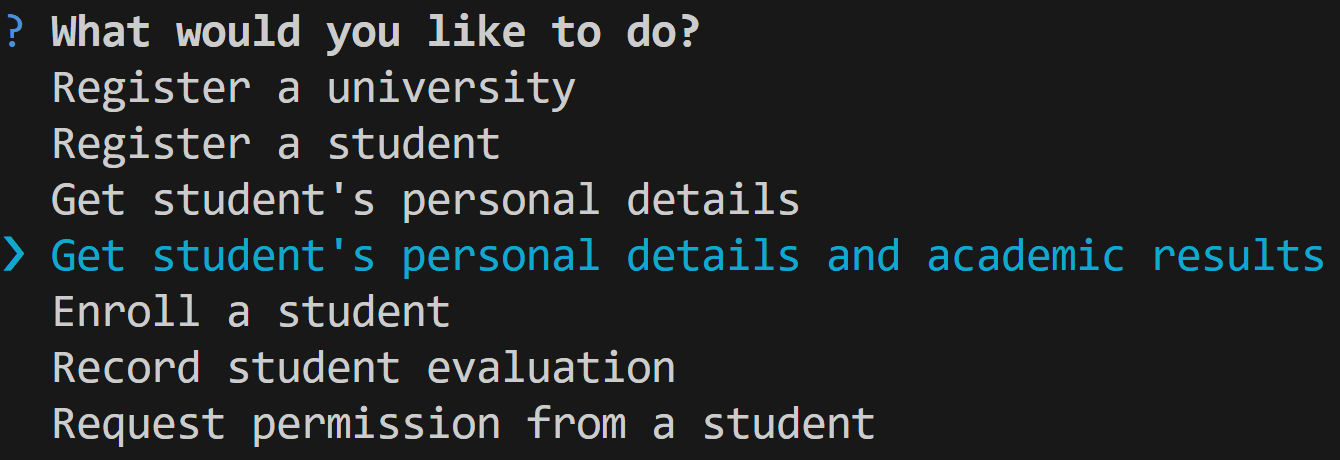
\includegraphics[width=\textwidth]{figures/CLI screen 1.png}
        \caption{Sliding menu}
        \label{sfig:cliDesign1}
    \end{subfigure}
    \hfill
    \begin{subfigure}{.60\textwidth}
        \centering
        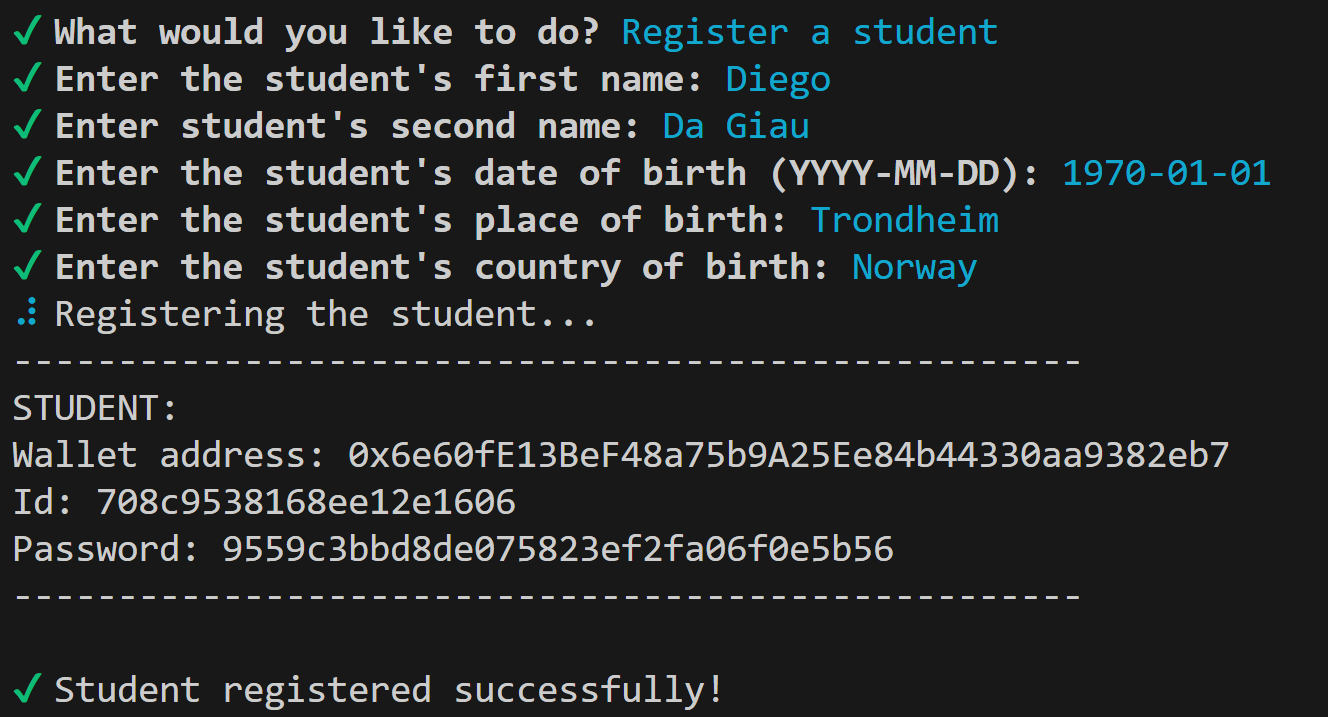
\includegraphics[width=\textwidth]{figures/CLI screen 2.png}
        \caption{User input and visual feedbacks}
        \label{sfig:cliDesign2}
    \end{subfigure}
    \caption[Different aspects of the \acrshort{cli} interface.]{Snapshots of the \acrshort{cli} interface}
    \label{fig:clifigs}
\end{figure}

\subsection{CLI Features}
The \acrshort{cli} exposes all the features outlined in \cref{fig:useCaseCli}. Users can:
\begin{itemize}
    \item Submit a request to register a university in the \acrshort{ew} system.
    \item Register a new student.
    \item Retrieve a student’s personal details.
    \item Retrieve a student’s details and academic results.
    \item Enrol a student in a new course.
    \item Evaluate a student.
    \item Request permissions from a student.
    \item Verify existing permissions.
\end{itemize}
Additionally, the \acrshort{cli} provides options to change the current university and exit the program.

\begin{figure}
  \centering
  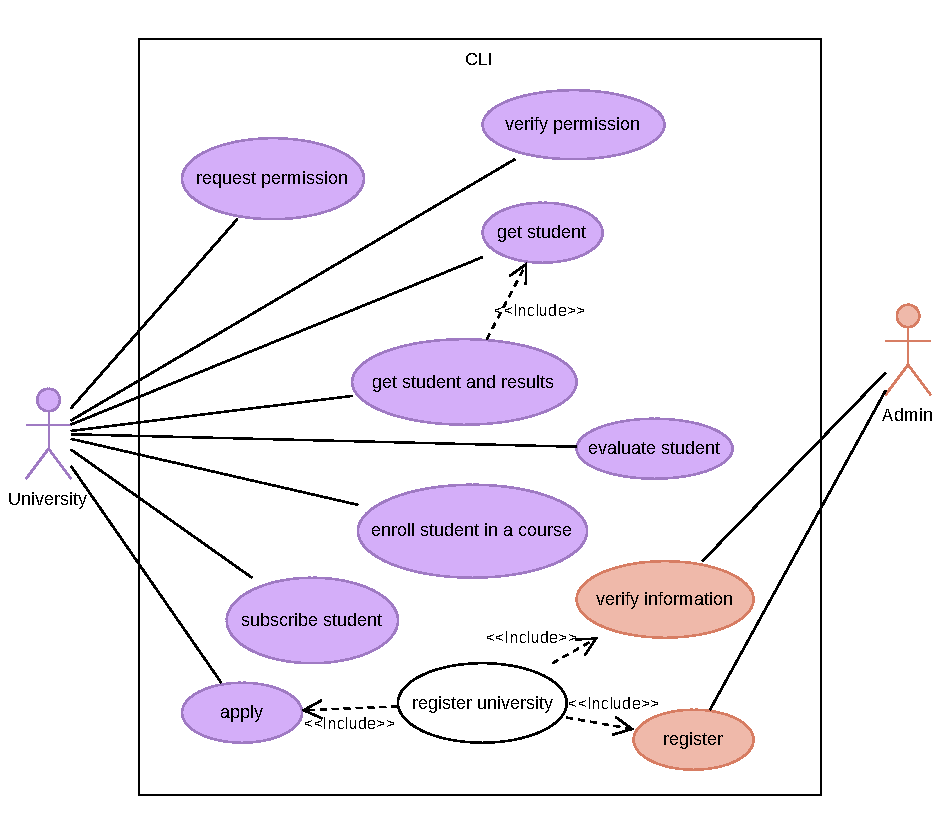
\includegraphics[width=0.8\textwidth]{figures/CLI use case diagram.pdf}
  \caption[\acrshort{cli} use case diagram]{Use case diagram representing the functionalities provided by the \acrshort{cli}.}
  \label{fig:useCaseCli}
\end{figure}

\subsubsection{Testing environment initialization}
Before performing any operation, the \acrshort{cli} must initialize a local blockchain test network by deploying the following smart contracts:
\begin{itemize}
    \item EntryPoint
    \item StudentDeployer
    \item UniversityDeployer
    \item Paymaster
    \item StudentsRegister
\end{itemize}
The \textit{Paymaster} contract then must also be funded to sponsor users' transactions.

In public testnets or in production networks, this initialization step would be unnecessary, as the contracts would already be deployed. Their addresses would be hardcoded in the \acrshort{cli}, \acrshort{sdk} and browser extension.

\subsubsection{University registration}
\label{sssec:applyEw}
To apply to the \acrshort{ew} system, a university must provide its name, country, and short name. Upon receiving these parameters, the \acrshort{cli} generates a random private key, which becomes the private key of the university's \acrshort{eoa}. The \acrshort{eoa} is then set as the active identity used to execute the subsequent operations on behalf of the university. Upon successful completion, the the \acrshort{cli} returns the generated private key, which is essential for accessing the its \acrshort{sca}. In a real \acrshort{lms}, this private key must be securely stored and used to initialize the \acrshort{eoa} wallet when interact with the \acrshort{sdk}. 

To enable immediate interaction with the EntryPoint contract on the local testnet, the \acrshort{cli} also funds the university's \acrshort{eoa}. This step is unnecessary in public or production networks, where the bundler covers transaction fees and is reimbursed by the Paymaster.

\subsubsection{Register a new student}
To register a student, the  university provides their name, surname, date of birth, place of birth and country of birth. The \acrshort{cli} then invokes the \acrshort{sdk} to create the student's smart account and credentials, which are returned to the university (\cref{sfig:cliDesign2}). The \acrshort{sca} address uniquely identifies the student and must be stored by the university, as it is required for all future interactions. 

The \acrshort{cli} also funds the student's \acrshort{eoa} for local testing. The wallet address is obtained from the login credentials, as explained for the browser extension in \cref{sec:browserExtensionDesign}.

\subsubsection{Student Information Retrieval}
To retrieve a student's personal information or full academic record, university must provide the student's smart account address. The \acrshort{cli} then returns the requested data.

\subsubsection{Enrol and evaluate}
To enrol or evaluate a student, the university must provide the smart account address and course code. Enrolment also requires the course name, number of \acrshort{ects} and degree course name. Evaluation requires the evaluation date and, optionally, the path to a certificate file. Since the \acrshort{sdk} allows enrolment in or evaluation of multiple courses at once, the \acrshort{cli} also supports submitting multiple records in a single command.     

\subsubsection{Permissions: Request and Verification}
To access or modify student's academic records, the university must request permission. The \acrshort{cli} requires the student's \acrshort{sca} address and the type of permission (read or write).
The \acrshort{cli} also includes the option to verify whether the university currently has read or write permission for a specific student.

\subsubsection{Changing University and Exiting the \acrshort{cli}}
These functionalities are unique to the \acrshort{cli} and are included for convenience. To change the active university, the user provides the private key of another registered university. To exit the \acrshort{cli}, the user selects the corresponding menu option.

\subsubsection{Administrator Functionalities}
The \acrshort{cli} also includes admin functionalities, as outlined  in \textit{FR 1} of \cref{tab:funcReq}, to facilitate system testing. Specifically, the administrator can:
\begin{itemize}
    \item Review the information submitted in university registration request.
    \item Approve and register universities in the system.
\end{itemize}
These functionalities are embedded within the university registration option. A university is automatically registered when its information is provided by the user during the registration process.

\subsection{Data validation}
All user input is validated using regular expressions and formatting rules. For instance, wallet addresses and private keys are validated based on length and structure\footnote{Private keys must start with \textit{0x} and be followed by 64 hexadecimal characters; addresses by 42.}. Strings are validated to fall within predefined length limits. Dates must follow the \textit{YYYY-MM-DD} format to avoid ambiguity and must be after January 1, 1970, as they are stored as Unix timestamps (unsigned integers). \acrshort{ects} values are checked to ensure they are valid integers or floating-point numbers within acceptable limits. Since the smart contracts store \acrshort{ects} as integers scaled by 100 (see \cref{sec:studentContract} for further details), the \acrshort{cli} ensures the values will not cause overflow during storage.